\newpage
\section{Multiplikation $a\cdot b$}

% ----------------------------------------------------------------------------
\subsection{Definition}
Die Multiplikation ist eine Rechenoperation der zweiten Stufe. Das Produkt zweier natürlicher Zahlen $n$ und $a$ entsteht durch das wiederholte Addieren des gleichen Summanden $a$ zum Ausgangswert Null:
\[
  n\cdot a := 0+\underbrace{a+a+\cdots+a}_{n-\text{mal}}
\]
Wenn in dieser Definition $n=0$ gesetzt wird, kommt $a$ gar nicht als Summand vor und das Resultat ist $0$.
\begin{theorem}
  \textbf{Multiplikation mit Null:} Das Produkt einer beliebigen Zahl $a$ und Null ist gleich Null.
  \[
    0 \cdot a = 0
  \]
\end{theorem}

% ----------------------------------------------------------------------------
\subsection{Schreib- und Sprechweise}
Die beiden Zahlen $a$ und $b$, welche multipliziert werden, heissen \textbf{Faktoren}, das Resultat $c$ heisst \textbf{Produkt}.

Für die Multiplikation wird das Zeichen $\cdot$ verwendet. Wir schreiben
\[
  a \cdot b = c
\]
und sagen «$a$ mal $b$ ist gleich $c$.» oder «Das Produkt von $a$ und $b$ ist gleich $c$.»
\begin{example}
  Das Produkt von Zwei und Drei ist gleich Sechs: $2 \cdot 3 = 6$
\end{example}

% ----------------------------------------------------------------------------
\subsection{Geometrische Interpretation}

Geometrisch entspricht das Produkt zweier Zahlen $a\cdot b$ dem Flächeninhalt eines Rechtecks mit den entsprechenden Seiten $a$ und $b$.

Das Produkt dreier Zahlen $a\cdot b\cdot c$ entspricht dem Volumen eines Quaders mit den Seiten $a$, $b$ und $c$.
\begin{center}
  \begin{tikzpicture}[scale=0.8]
    \tkzText(2.5,3.5){$a\cdot b$}
    \tkzDefPoint(0,0){A1}
    \tkzDefPoint(5,0){A2}
    \tkzDefPoint(5,3){A3}
    \tkzDefPoint(0,3){A4}
    \tkzDrawPolygon[fill=lightgreen](A1,A2,A3,A4)
    \tkzLabelLine[below](A1,A2){$a$}
    \tkzLabelLine[left](A1,A4){$b$}
    \foreach \y in {0,...,3}{\tkzDrawSegment({0,\y},{5,\y})}
    \foreach \x in {0,...,5}{\tkzDrawSegment({\x,0},{\x,3})}

    \tkzText(10,3.5){$a\cdot b\cdot c$}
    \tkzDefPoint(7,0){B1}
    \tkzDefPoint(12,0){B2}
    \tkzDefPoint(12,2){B3}
    \tkzDefPoint(7,2){B4}
    \tkzDefPoint(13,1){B5}
    \tkzDefPoint(13,3){B6}
    \tkzDefPoint(8,3){B7}
    \tkzDrawPolygon[fill=lightgreen](B1,B2,B3,B4)
    \tkzDrawPolygon[fill=lightgreen](B2,B5,B6,B3)
    \tkzDrawPolygon[fill=lightgreen](B3,B6,B7,B4)
    \tkzLabelLine[below](B1,B2){$a$}
    \tkzLabelLine[left](B1,B4){$c$}
    \tkzLabelLine[below right](B2,B5){$b$}

    \tkzDrawSegment({12.33,0.33},{12.33,2.33})
    \tkzDrawSegment({12.67,0.67},{12.67,2.67})
    \tkzDrawSegment({7.33,2.33},{12.33,2.33})
    \tkzDrawSegment({7.67,2.67},{12.67,2.67})

    \foreach \y in {0,...,2}{\tkzDrawSegment({7,\y},{12,\y})}
    \foreach \y in {0,...,2}{\tkzDrawSegment({12,\y},{13,\y+1})}
    \foreach \x in {7,...,12}{\tkzDrawSegment({\x,0},{\x,2})}
    \foreach \x in {7,...,12}{\tkzDrawSegment({\x,2},{\x+1,3})}
  \end{tikzpicture}
\end{center}

% ----------------------------------------------------------------------------
\subsection{Kommutativgesetz}

Anhand der geometrischen Interpretation wird ersichtlich, dass auch für die Multiplikation das Kommutativgesetz gelten muss. Das Vertauschen der beiden Faktoren entspricht dem Vertauschen der beiden Seitenlängen eines Rechtecks, was einer Drehung um \ang{90} entspricht. Die Fläche des Rechtecks und somit das Produkt verändert sich dabei nicht.
\begin{center}
  \begin{tikzpicture}[scale=0.8]
    \tkzDefPoint(0,0){A1}
    \tkzDefPoint(4,0){A2}
    \tkzDefPoint(4,3){A3}
    \tkzDefPoint(0,3){A4}
    \tkzDrawPolygon[fill=lightgreen](A1,A2,A3,A4)
    \tkzLabelLine[below](A1,A2){$a$}
    \tkzLabelLine[left](A1,A4){$b$}
    \foreach \y in {0,...,3}{\tkzDrawSegment({0,\y},{4,\y})}
    \foreach \x in {0,...,4}{\tkzDrawSegment({\x,0},{\x,3})}

    \tkzDefPoint(7,-0.5){B1}
    \tkzDefPoint(10,-0.5){B2}
    \tkzDefPoint(10,3.5){B3}
    \tkzDefPoint(7,3.5){B4}
    \tkzDrawPolygon[fill=lightgreen](B1,B2,B3,B4)
    \tkzLabelLine[below](B1,B2){$b$}
    \tkzLabelLine[left](B1,B4){$a$}
    \foreach \y in {0,...,4}{\tkzDrawSegment({7,\y-0.5},{10,\y-0.5})}
    \foreach \x in {0,...,3}{\tkzDrawSegment({\x+7,-0.5},{\x+7,3.5})}
  \end{tikzpicture}
\end{center}
\begin{theorem}
  \textbf{Kommutativgesetz.} Die Faktoren einer Multiplikation dürfen vertauscht werden, ohne dass sich der Wert des Produkts ändert:
  \[
    a \cdot b = b \cdot a
  \]
\end{theorem}

% ----------------------------------------------------------------------------
\subsection{Assoziativgesetz}
Das Volumen eines Quaders ergibt sich aus der Grundfläche multipliziert mit der Höhe. Je nach Orientierung des Quaders ergibt sich somit eine andere Formel für das gleiche Volumen. Wird bei der rechten Formel das Kommutativgesetz angewendet, ergibt sich daraus das Assoziativgesetz für die Multiplikation.
\begin{center}
  \begin{tikzpicture}[scale=0.8]
    \tkzDefPoint(0,0){A1}
    \tkzDefPoint(4,0){A2}
    \tkzDefPoint(4,2){A3}
    \tkzDefPoint(0,2){A4}
    \tkzDefPoint(5,1){A5}
    \tkzDefPoint(5,3){A6}
    \tkzDefPoint(1,3){A7}
    \tkzDrawPolygon[fill=lightgreen](A1,A2,A3,A4)
    \tkzDrawPolygon[fill=lightgreen](A2,A5,A6,A3)
    \tkzDrawPolygon[fill=lightgreen](A3,A6,A7,A4)
    \tkzLabelLine[below](A1,A2){$a$}
    \tkzLabelLine[left](A1,A4){$c$}
    \tkzLabelLine[below right](A2,A5){$b$}

    \tkzDrawSegment({4.33,0.33},{4.33,2.33})
    \tkzDrawSegment({4.67,0.67},{4.67,2.67})
    \tkzDrawSegment({0.33,2.33},{4.33,2.33})
    \tkzDrawSegment({0.67,2.67},{4.67,2.67})

    \foreach \y in {0,...,2}{\tkzDrawSegment({0,\y},{4,\y})}
    \foreach \y in {0,...,2}{\tkzDrawSegment({4,\y},{5,\y+1})}
    \foreach \x in {0,...,4}{\tkzDrawSegment({\x,0},{\x,2})}
    \foreach \x in {0,...,4}{\tkzDrawSegment({\x,2},{\x+1,3})}

    \tkzDefPoint(7,0){B1}
    \tkzDefPoint(10,0){B2}
    \tkzDefPoint(10,4){B3}
    \tkzDefPoint(7,4){B4}
    \tkzDefPoint(10.67,0.67){B5}
    \tkzDefPoint(10.67,4.67){B6}
    \tkzDefPoint(7.67,4.67){B7}
    \tkzDrawPolygon[fill=lightgreen](B1,B2,B3,B4)
    \tkzDrawPolygon[fill=lightgreen](B2,B5,B6,B3)
    \tkzDrawPolygon[fill=lightgreen](B3,B6,B7,B4)
    \tkzLabelLine[below](B1,B2){$b$}
    \tkzLabelLine[left](B1,B4){$a$}
    \tkzLabelLine[below right](B2,B5){$c$}

    \tkzDrawSegment({10.33,0.33},{10.33,4.33})
    \tkzDrawSegment({10.67,0.67},{10.67,4.67})
    \tkzDrawSegment({7.33,4.33},{10.33,4.33})
    \tkzDrawSegment({7.67,4.67},{10.67,4.67})

    \foreach \y in {0,...,4}{\tkzDrawSegment({7,\y},{10,\y})}
    \foreach \y in {0,...,4}{\tkzDrawSegment({10,\y},{10.67,\y+0.67})}
    \foreach \x in {7,...,10}{\tkzDrawSegment({\x,0},{\x,4})}
    \foreach \x in {7,...,10}{\tkzDrawSegment({\x,4},{\x+0.67,4.67})}

    \tkzText(3,3.5){$a\cdot b\cdot c$}
    \tkzText[black](9,5.2){$b\cdot c\cdot a = a\cdot (b\cdot c)$}
  \end{tikzpicture}
\end{center}
\begin{theorem}
  \textbf{Assoziativgesetz.} Mehrere Multiplikationen dürfen in beliebiger Reihenfolge ausgeführt werden, ohne dass sich der Wert des Produkts ändert:
  \[
    a \cdot b \cdot c = (a \cdot b) \cdot c = a \cdot (b \cdot c)
  \]
\end{theorem}

% ----------------------------------------------------------------------------
\subsection{Neutralität der Eins}

Die Eins hat bezüglich der Multiplikation eine besondere Stellung. Das Multiplizieren mit Eins verändert den Wert nicht.
\begin{theorem}
  \textbf{Neutralität der Eins.} Eine Zahl kann mit Eins multipliziert werden, ohne dass sich der Wert ändert:
  \[
    a \cdot 1 = 1 \cdot a = a
  \]
\end{theorem}


% ----------------------------------------------------------------------------
\subsection{Distributivgesetz}
Das Distributivgesetz verbindet die Addition und die Multiplikation. Es kann ebenfalls durch eine geometrische Überlegung begründet werden. Wird das Rechteck mit den Seiten $a$ und $b$ und das Rechteck mit den Seiten $a$ und $c$ zusammengesetzt, so ergibt sich ein Rechteck mit den Seiten $a$ und $b+c$, welches die gleiche Fläche wie die beiden ersten Rechtecke hat.
\begin{center}
  \begin{tikzpicture}[scale=0.8]
    \tkzText(3,3.5){$a\cdot b+a\cdot c$}
    \tkzDefPoint(0,0){A1}
    \tkzDefPoint(3,0){A2}
    \tkzDefPoint(3,3){A3}
    \tkzDefPoint(0,3){A4}
    \tkzDrawPolygon[fill=lightgreen](A1,A2,A3,A4)
    \tkzLabelLine[below](A1,A2){$b$}
    \tkzLabelLine[left](A1,A4){$a$}
    \foreach \y in {0,...,3}{\tkzDrawSegment({0,\y},{3,\y})}
    \foreach \x in {0,...,3}{\tkzDrawSegment({\x,0},{\x,3})}

    \tkzDefPoint(4,0){B1}
    \tkzDefPoint(6,0){B2}
    \tkzDefPoint(6,3){B3}
    \tkzDefPoint(4,3){B4}
    \tkzDrawPolygon[fill=lightgreen](B1,B2,B3,B4)
    \tkzLabelLine[below](B1,B2){$c$}
    \tkzLabelLine[left](B1,B4){$a$}
    \foreach \y in {0,...,3}{\tkzDrawSegment({4,\y},{6,\y})}
    \foreach \x in {4,...,6}{\tkzDrawSegment({\x,0},{\x,3})}

    \tkzText(10.5,3.5){$a\cdot(b+c)$}
    \tkzDefPoint(8,0){C1}
    \tkzDefPoint(13,0){C2}
    \tkzDefPoint(13,3){C3}
    \tkzDefPoint(8,3){C4}
    \tkzDrawPolygon[fill=lightgreen](C1,C2,C3,C4)
    \tkzLabelLine[below](C1,C2){$b+c$}
    \tkzLabelLine[left](C1,C4){$a$}
    \foreach \y in {0,...,3}{\tkzDrawSegment({8,\y},{13,\y})}
    \foreach \x in {8,...,13}{\tkzDrawSegment({\x,0},{\x,3})}
  \end{tikzpicture}
\end{center}

\begin{theorem}
  \textbf{Distributivgesetz.} Eine Summe wird mit einem Faktor $a$ multipliziert, indem jeder Summand mit $a$ multipliziert wird.
  \[
    a \cdot (b + c) = a \cdot b + a \cdot c
  \]
\end{theorem}
